\documentclass[tikz,border=10pt]{standalone}
% Shared style for all project diagrams
\usepackage{amsmath,amssymb}
\usetikzlibrary{positioning,arrows.meta,calc,fit,decorations.pathreplacing}
\renewcommand{\familydefault}{\sfdefault}
\definecolor{accent}{RGB}{42,120,214}
\definecolor{lblue}{RGB}{234,242,252}
\definecolor{card}{RGB}{247,247,245}
\definecolor{ink}{RGB}{17,17,17}
\definecolor{gray52}{RGB}{82,81,78}
\definecolor{dblue}{RGB}{13,54,107}
\tikzset{
  box/.style={draw=accent, thick, rounded corners=3pt, fill=lblue, align=center,
              minimum height=1.05cm, inner sep=6pt, text=ink},
  plain/.style={draw=gray52!60, thick, rounded corners=3pt, fill=card, align=center,
              minimum height=1.05cm, inner sep=6pt, text=ink},
  ghost/.style={align=center, text=gray52, font=\footnotesize},
  arr/.style={-{Stealth[length=2.6mm]}, very thick, draw=accent},
  garr/.style={-{Stealth[length=2.6mm]}, thick, draw=gray52},
  lbl/.style={font=\footnotesize, text=gray52, align=center},
}

\begin{document}
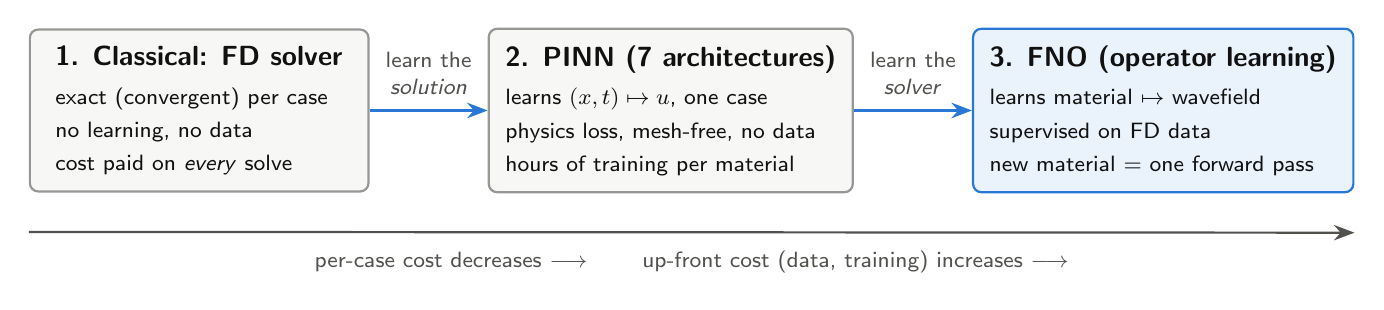
\begin{tikzpicture}[node distance=0.7cm and 1.5cm]
  \node[plain, minimum width=4.3cm, align=left] (fd)
    {\textbf{1. Classical: FD solver}\\[2pt]
     {\footnotesize exact (convergent) per case}\\
     {\footnotesize no learning, no data}\\
     {\footnotesize cost paid on \emph{every} solve}};
  \node[plain, right=of fd, minimum width=4.3cm, align=left] (pinn)
    {\textbf{2. PINN (7 architectures)}\\[2pt]
     {\footnotesize learns $(x,t)\mapsto u$, one case}\\
     {\footnotesize physics loss, mesh-free, no data}\\
     {\footnotesize hours of training per material}};
  \node[box, right=of pinn, minimum width=4.3cm, align=left] (fno)
    {\textbf{3. FNO (operator learning)}\\[2pt]
     {\footnotesize learns material $\mapsto$ wavefield}\\
     {\footnotesize supervised on FD data}\\
     {\footnotesize new material $=$ one forward pass}};

  \draw[arr] (fd) -- (pinn) node[midway, lbl, above=2pt] {learn the\\ \emph{solution}};
  \draw[arr] (pinn) -- (fno) node[midway, lbl, above=2pt] {learn the\\ \emph{solver}};

  \draw[garr] ($(fd.south west)+(0,-0.5)$) -- ($(fno.south east)+(0,-0.5)$)
    node[midway, lbl, below=3pt]
    {per-case cost decreases $\longrightarrow$ \qquad up-front cost (data, training) increases $\longrightarrow$};
\end{tikzpicture}
\end{document}
